\documentclass[11pt]{article}
\usepackage[margin=1in]{geometry}
\usepackage{booktabs}
\usepackage{tabularx}
\usepackage{float}
\usepackage{xcolor}
\usepackage{siunitx}
\usepackage{graphicx}
\usepackage{caption}
\usepackage{hyperref}
\usepackage{enumitem}
\setlist{nosep}
\hypersetup{colorlinks=true,linkcolor=black,urlcolor=blue}

\newcommand{\pass}{\textcolor{green!50!black}{\textbf{PASS}}}
\newcommand{\fail}{\textcolor{red!70!black}{\textbf{FAIL}}}

\title{2.4\,GHz FMCW Radar --- Horn Antenna Simulation}
\author{David Brown}
\date{October 2026}

\begin{document}
\maketitle

\noindent The horn antenna was simulated in Ansys HFSS (Student 2025 R2). Nothing has been built yet. Plots are in Section~\ref{sec:figs}.

\section{Results}

Pyramidal horn on WR-340, mouth $263.8 \times 193.1$\,mm, coax probe feed.
Band: 2400--2483.5\,MHz.

\begin{table}[H]
\centering
\small
\begin{tabularx}{\linewidth}{>{\raggedright\arraybackslash}X>{\raggedright\arraybackslash}p{3.3cm}>{\raggedright\arraybackslash}p{2.6cm}l}
\toprule
Check & Result & Requirement & \\
\midrule
Match (S11), worst in band, original probe (28 / 43.7\,mm) & $-5.2$\,dB & $\le -10$\,dB & \fail \\
Match (S11), worst in band, final probe (27 / 17.7\,mm) & $-24.3$\,dB & $\le -10$\,dB & \pass \\
Gain at 2.400 / 2.442 / 2.483\,GHz & 13.24 / 13.24 / 13.27\,dBi & 12.5--14\,dBi & \pass \\
Beamwidth, E / H plane & $34.4^\circ$ / $36.4^\circ$ & theory $33.4^\circ$ / $35.2^\circ$ & \pass \\
TX $\to$ RX leakage, horns 290\,mm apart & $-49.4$\,dB & $\le -35$\,dB & \pass \\
Match with probe off by $\pm1$\,mm & $-14.5$\,dB & $\le -10$\,dB & \pass \\
Mesh check (8.8k / 11.9k / 28.8k cells) & 0.14\,dB gain spread & $\le 0.2$\,dB & \pass \\
Copper walls vs.\ perfect conductor & $+0.01$\,dB gain & $\le 0.2$\,dB & \pass \\
\bottomrule
\end{tabularx}
\end{table}

\noindent\textbf{Change made:} probe moved from 28\,mm long, 43.7\,mm from the back wall, to
27\,mm long, 17.7\,mm from the back wall (picked from a 1\,mm sweep of 57 runs).

\section{Summary}
All checks pass after the probe move (27\,mm long, 17.7\,mm from the back wall).

\clearpage
\section{Figures}\label{sec:figs}

\begin{figure}[H]\centering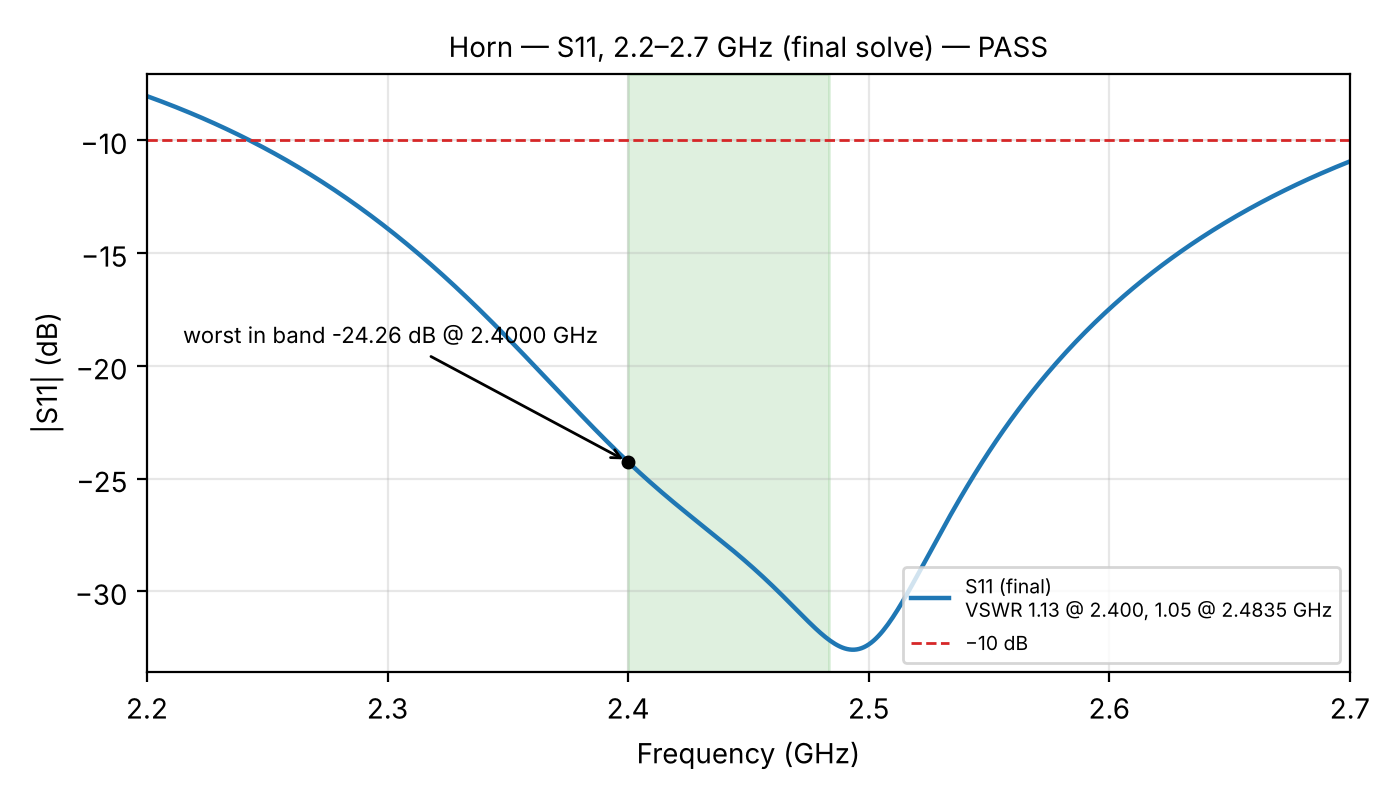
\includegraphics[width=0.85\linewidth,height=0.4\textheight,keepaspectratio]{figures/hfss/s11}\caption{Match (S11) across the band, final probe}\end{figure}
\begin{figure}[H]\centering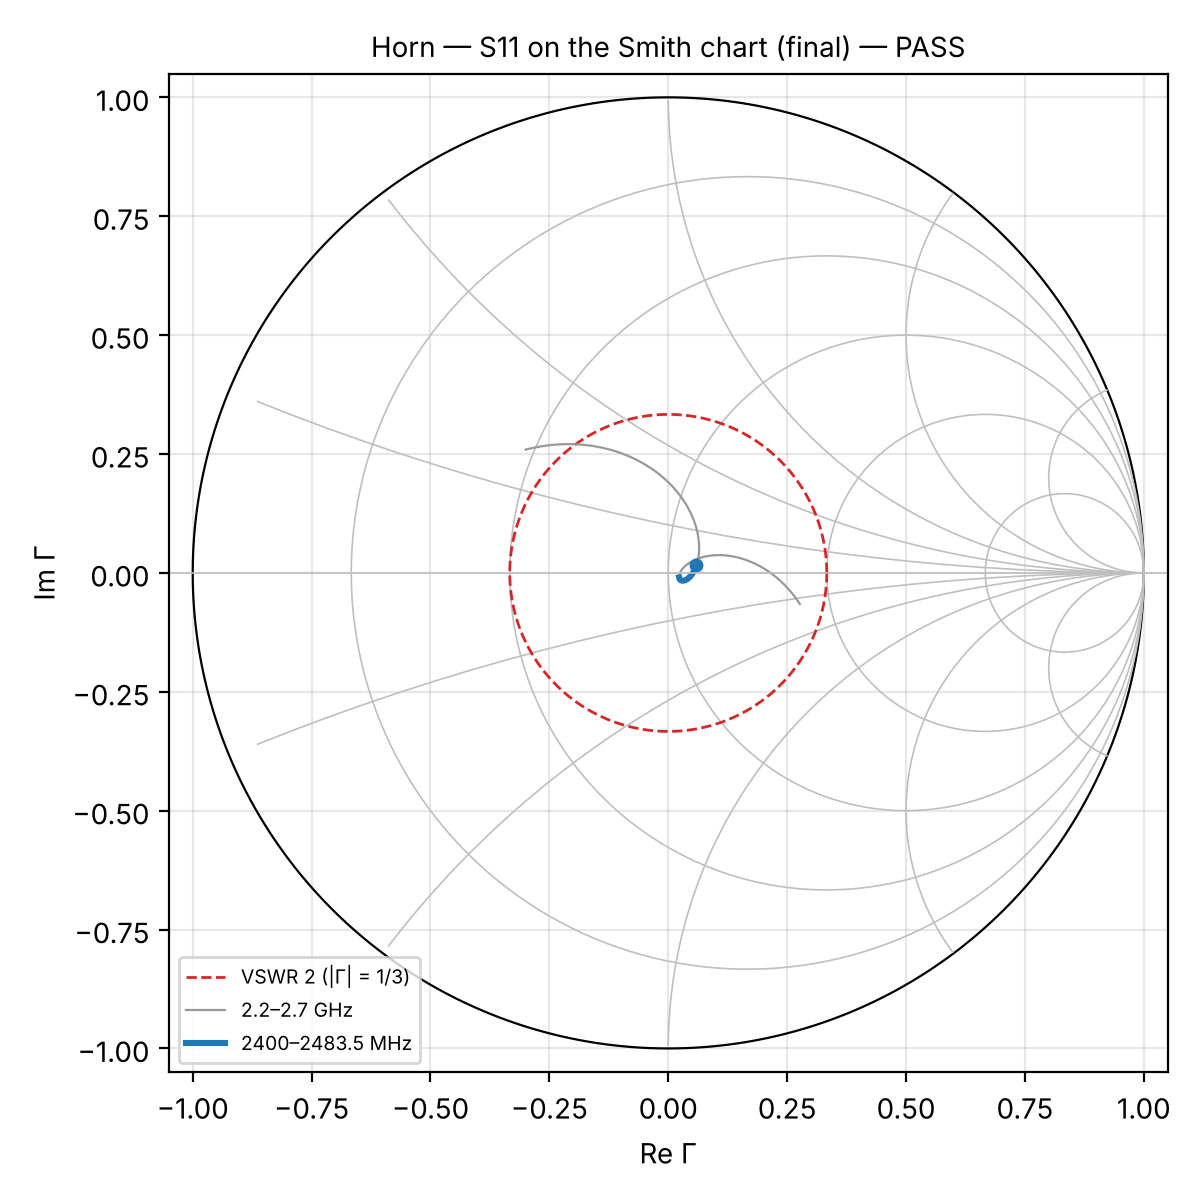
\includegraphics[width=0.85\linewidth,height=0.4\textheight,keepaspectratio]{figures/hfss/smith}\caption{Smith chart, final probe}\end{figure}
\begin{figure}[H]\centering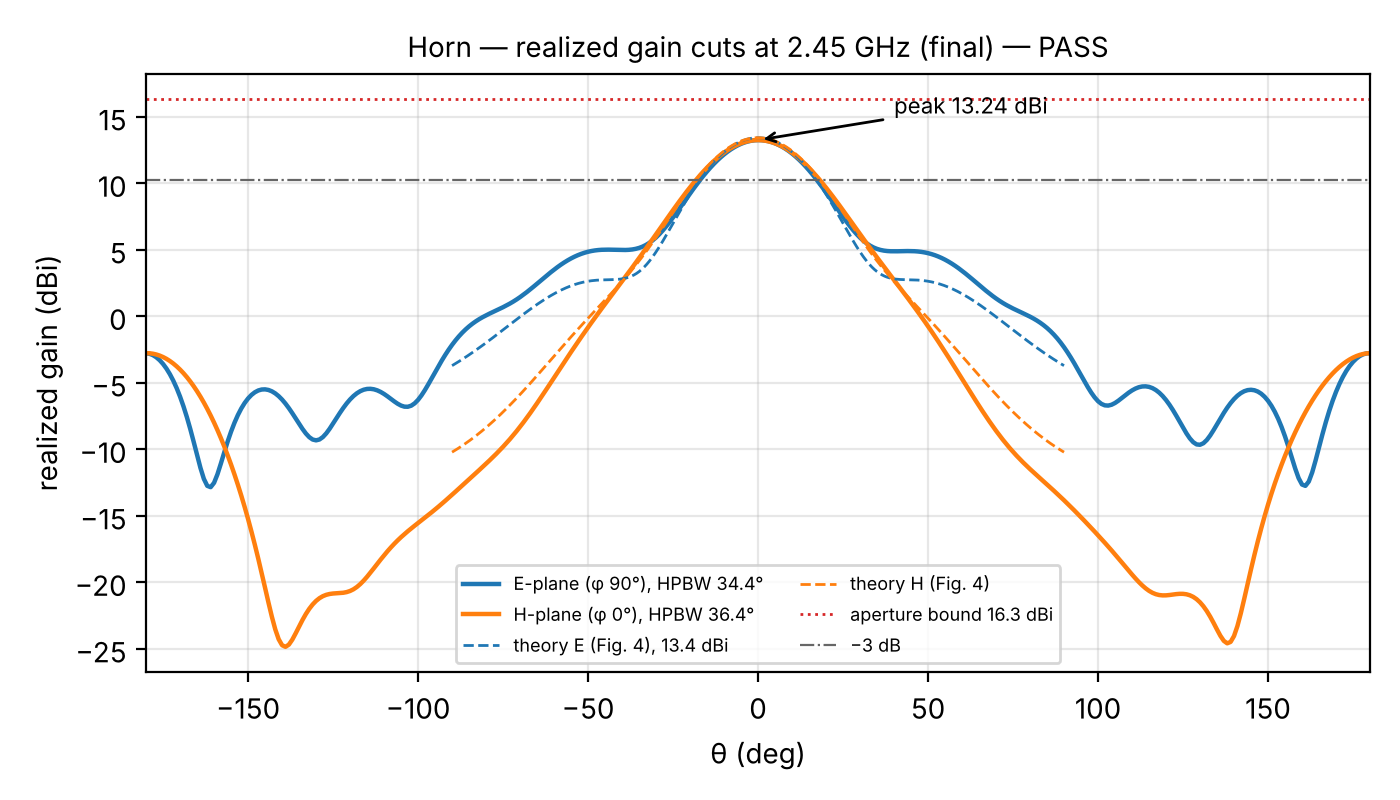
\includegraphics[width=0.85\linewidth,height=0.4\textheight,keepaspectratio]{figures/hfss/patterns}\caption{Gain patterns, E and H plane}\end{figure}
\begin{figure}[H]\centering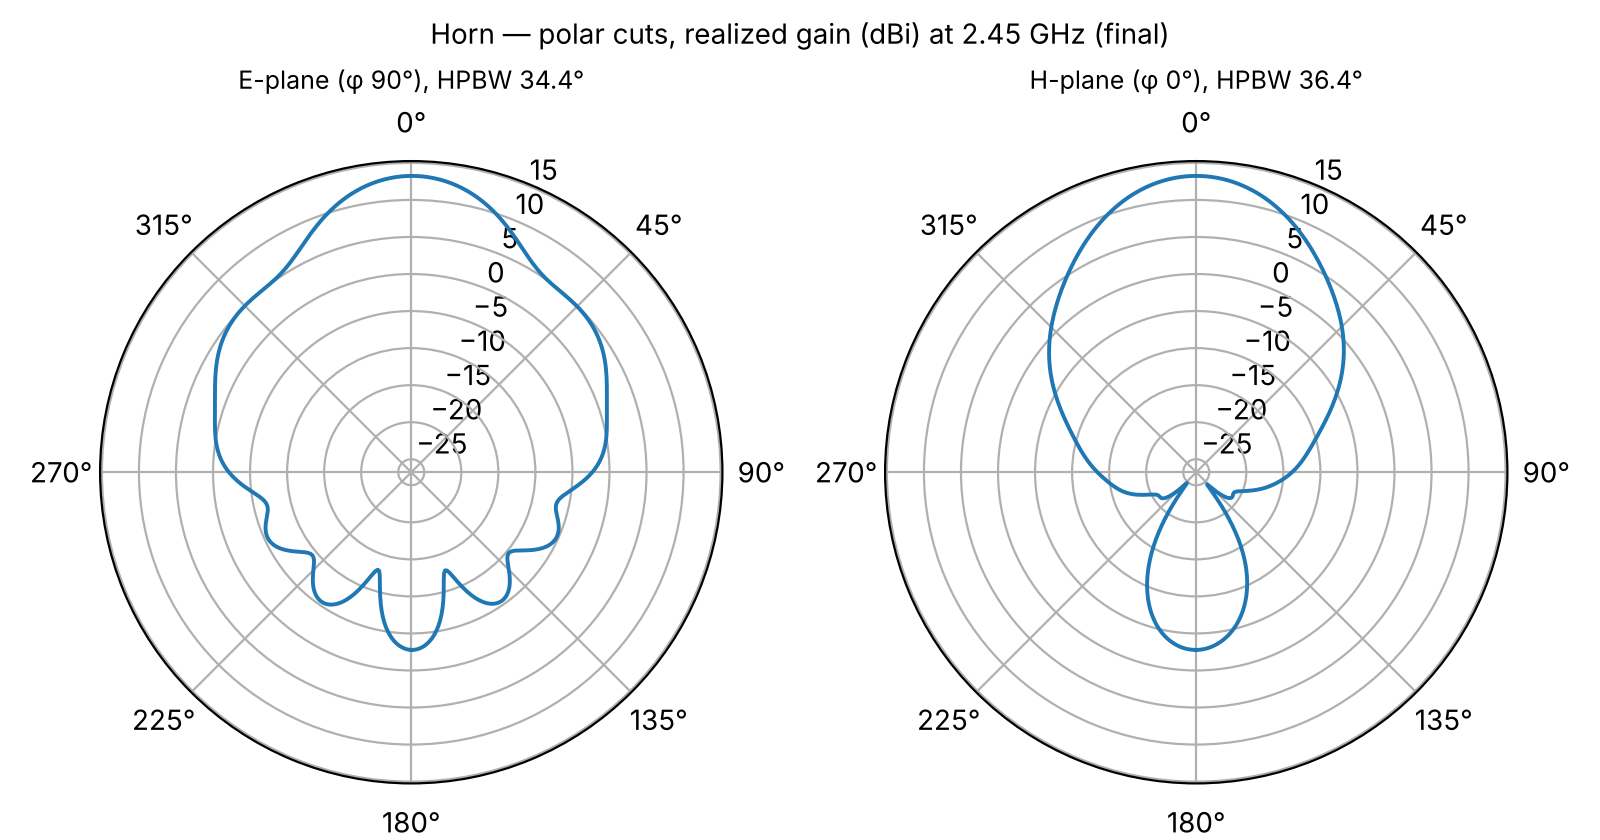
\includegraphics[width=0.85\linewidth,height=0.4\textheight,keepaspectratio]{figures/hfss/patterns_polar}\caption{Gain patterns, polar}\end{figure}
\begin{figure}[H]\centering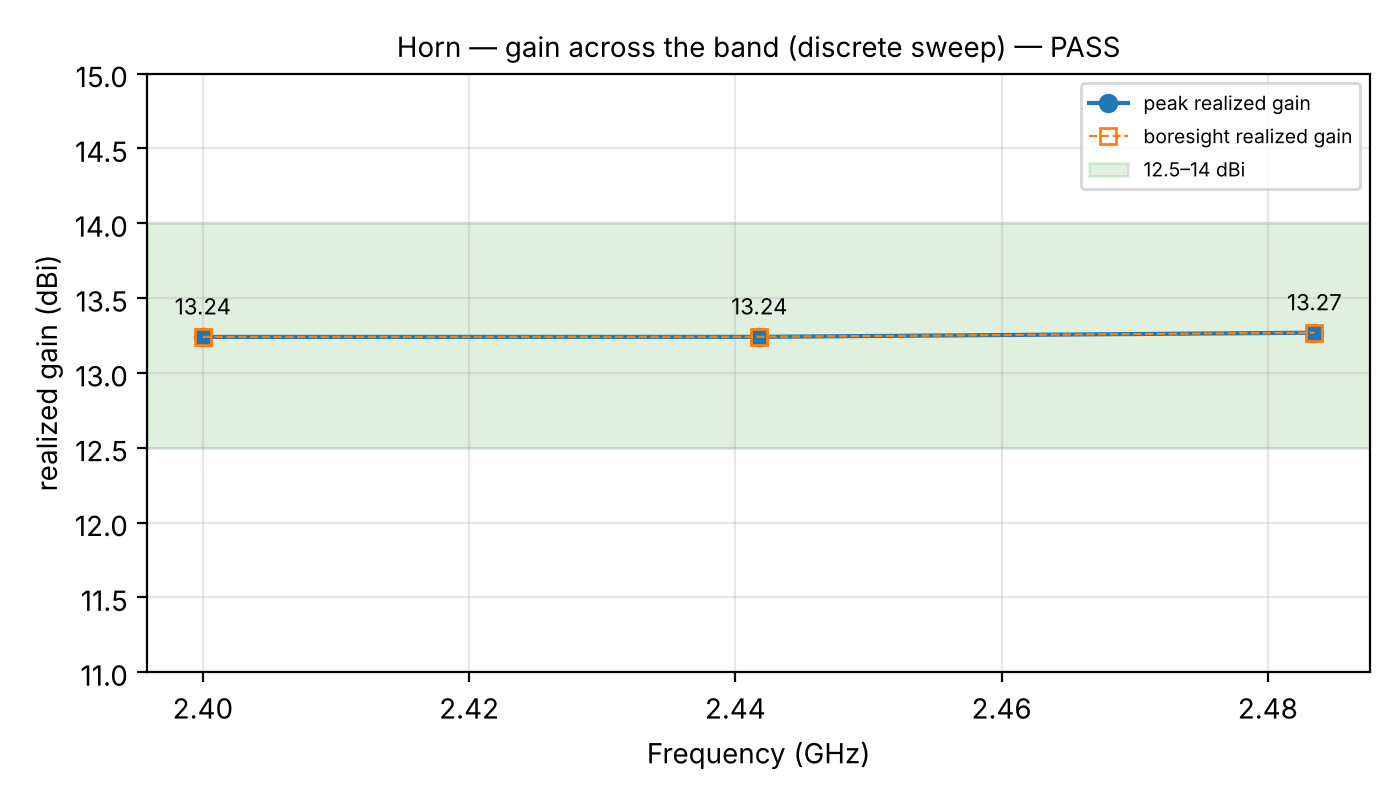
\includegraphics[width=0.85\linewidth,height=0.4\textheight,keepaspectratio]{figures/hfss/gain_vs_freq}\caption{Gain straight ahead across the band}\end{figure}
\begin{figure}[H]\centering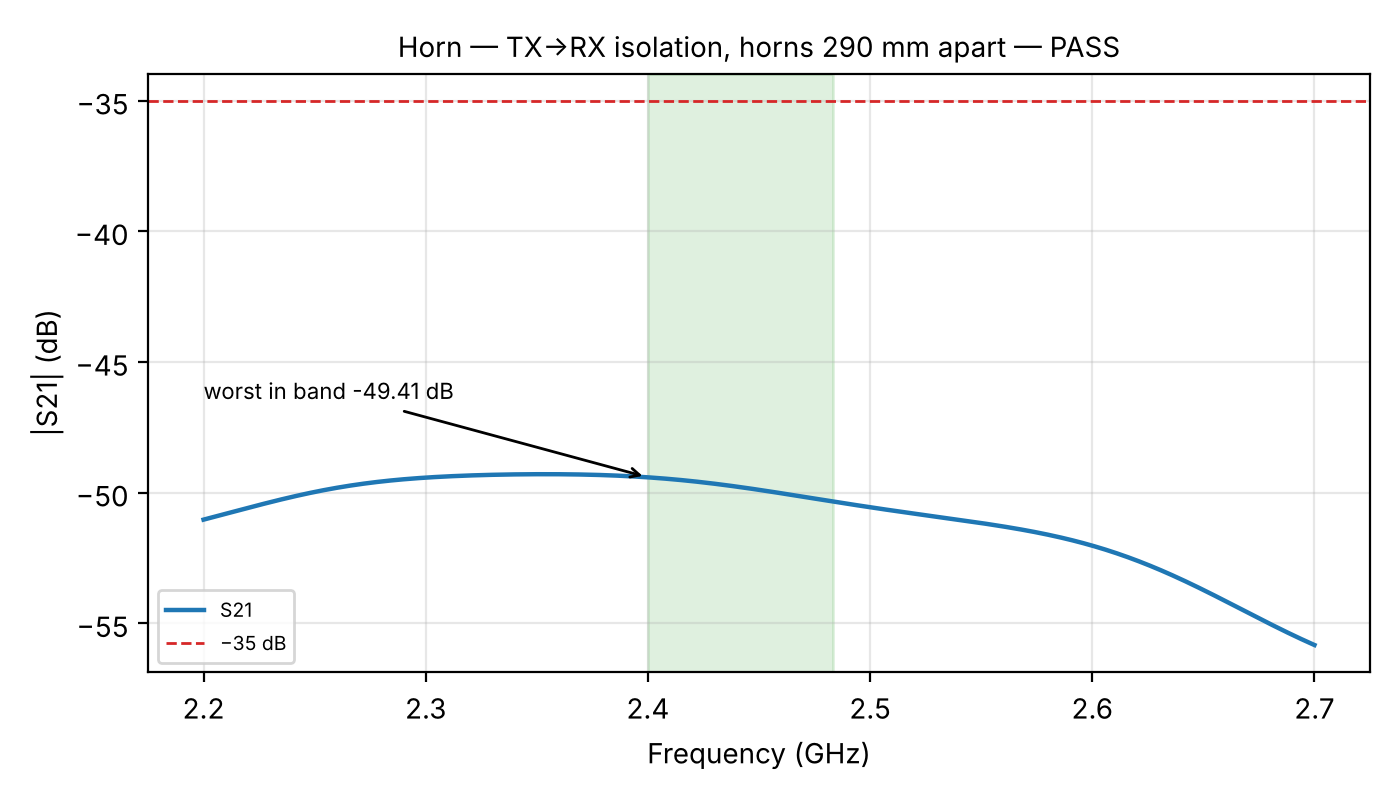
\includegraphics[width=0.85\linewidth,height=0.4\textheight,keepaspectratio]{figures/hfss/isolation}\caption{TX to RX leakage, horns 290 mm apart}\end{figure}
\begin{figure}[H]\centering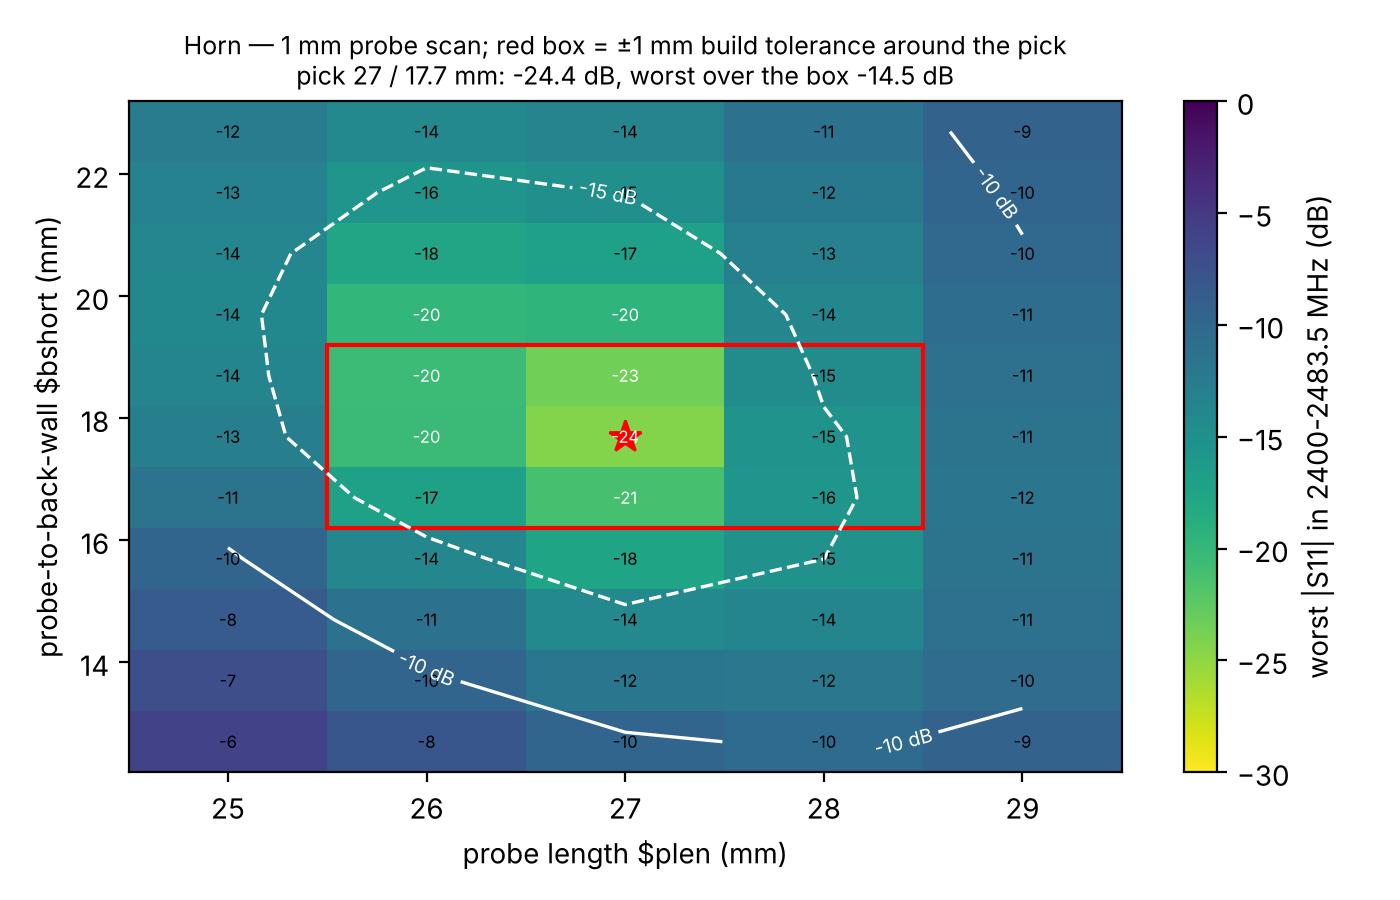
\includegraphics[width=0.85\linewidth,height=0.4\textheight,keepaspectratio]{figures/hfss/scan_heatmap}\caption{1 mm probe sweep: worst match in band}\end{figure}
\begin{figure}[H]\centering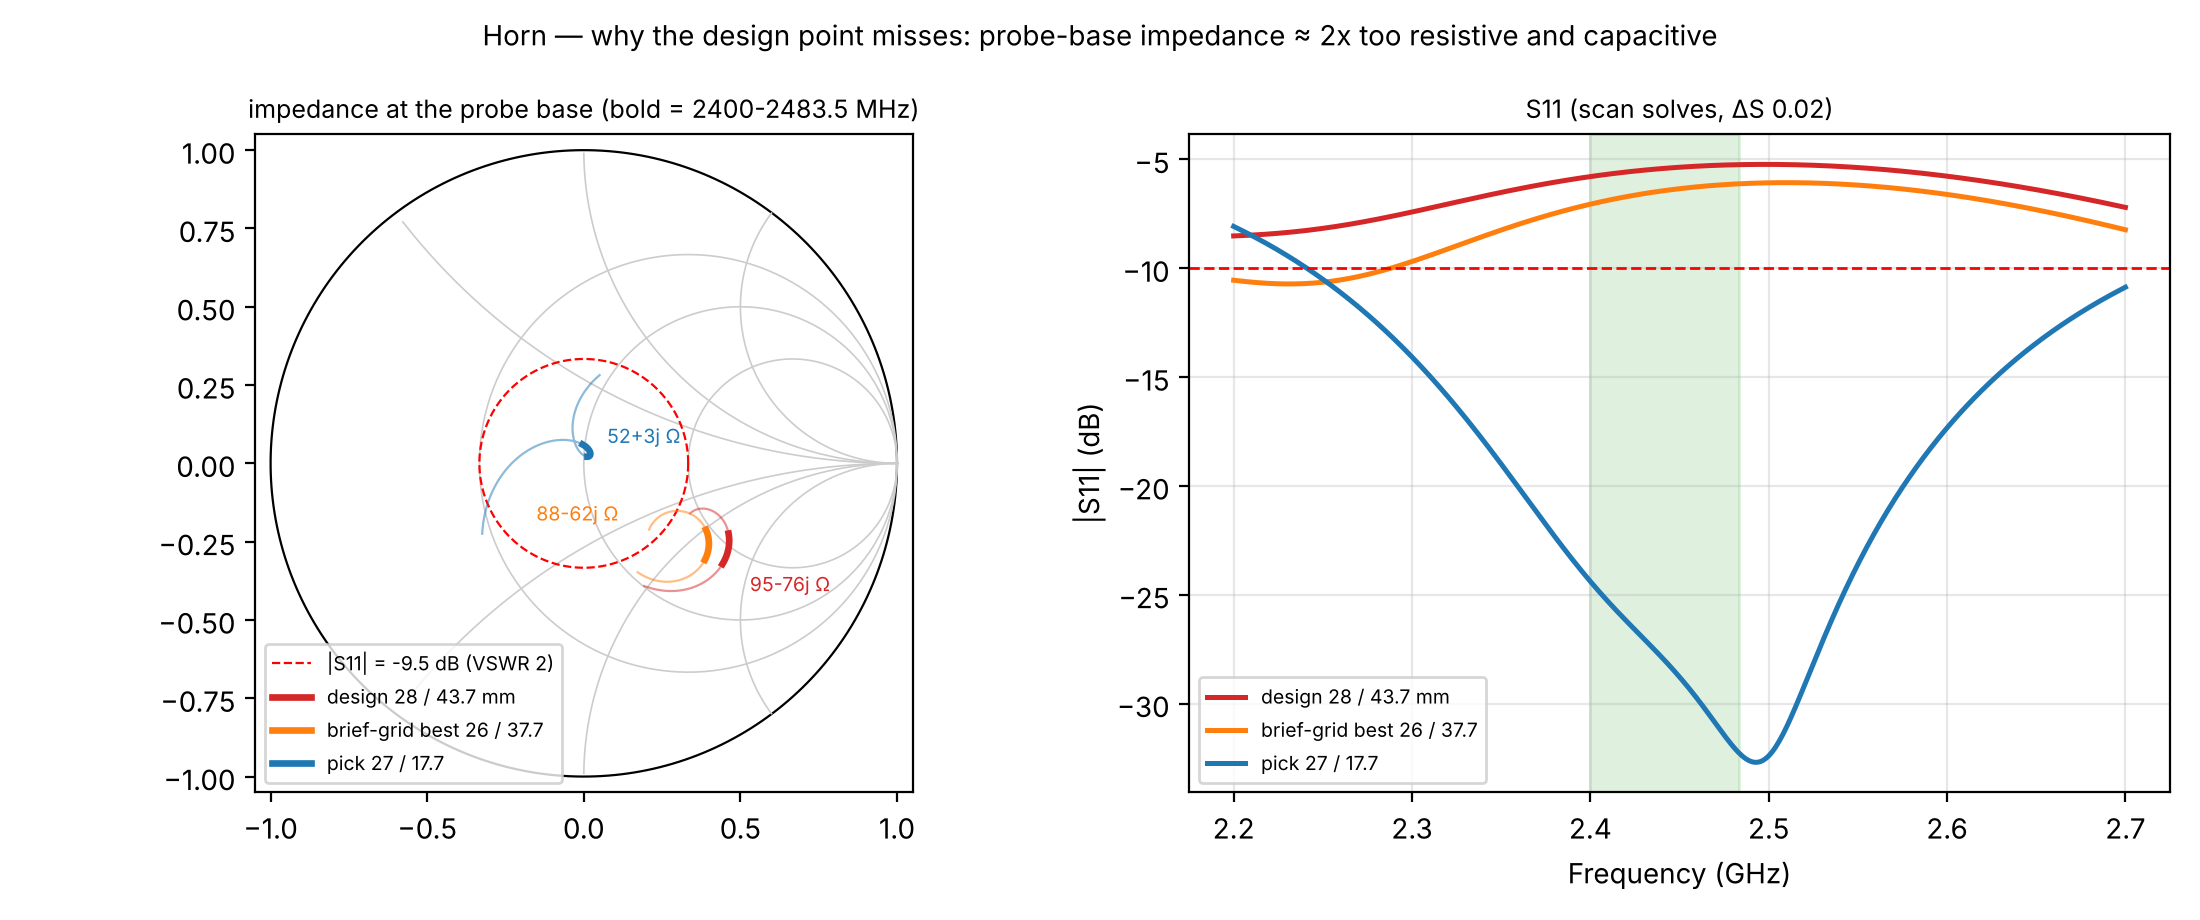
\includegraphics[width=0.85\linewidth,height=0.4\textheight,keepaspectratio]{figures/hfss/scan_diagnosis}\caption{Why the original probe position didn't match}\end{figure}
\begin{figure}[H]\centering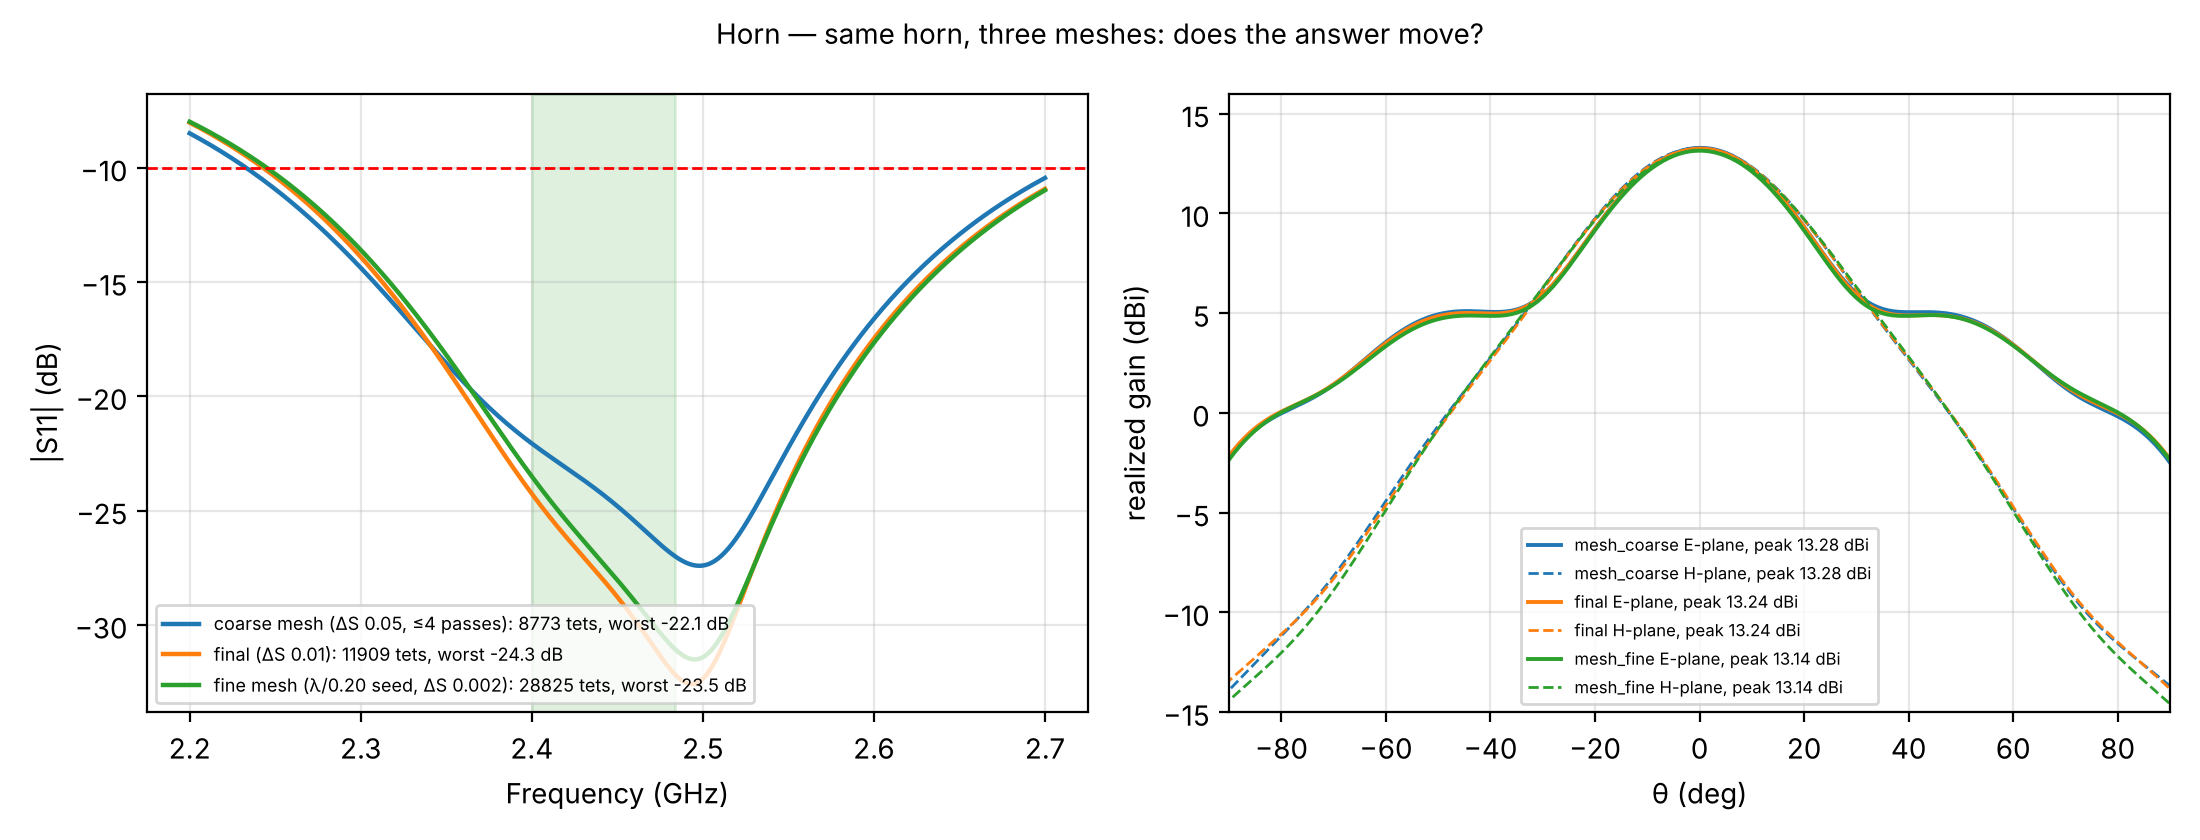
\includegraphics[width=0.85\linewidth,height=0.4\textheight,keepaspectratio]{figures/hfss/robust_mesh}\caption{Mesh check}\end{figure}
\begin{figure}[H]\centering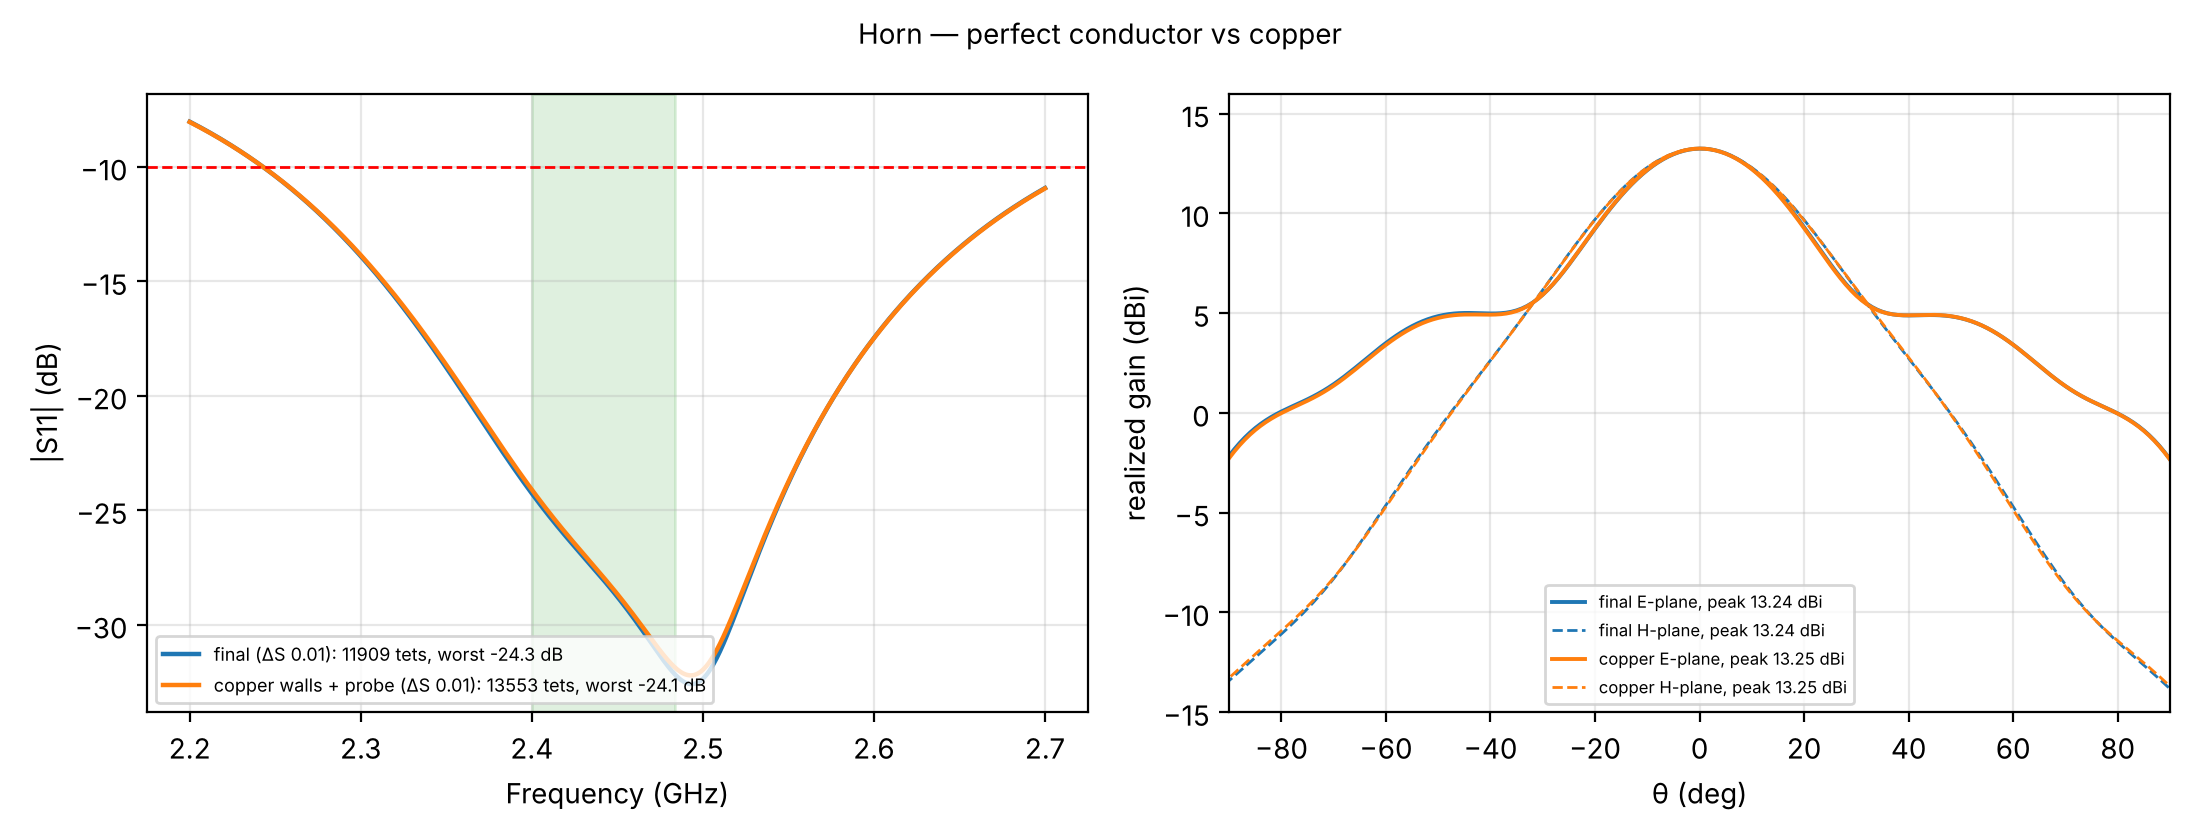
\includegraphics[width=0.85\linewidth,height=0.4\textheight,keepaspectratio]{figures/hfss/robust_copper}\caption{Copper vs. perfect conductor}\end{figure}
\begin{figure}[H]\centering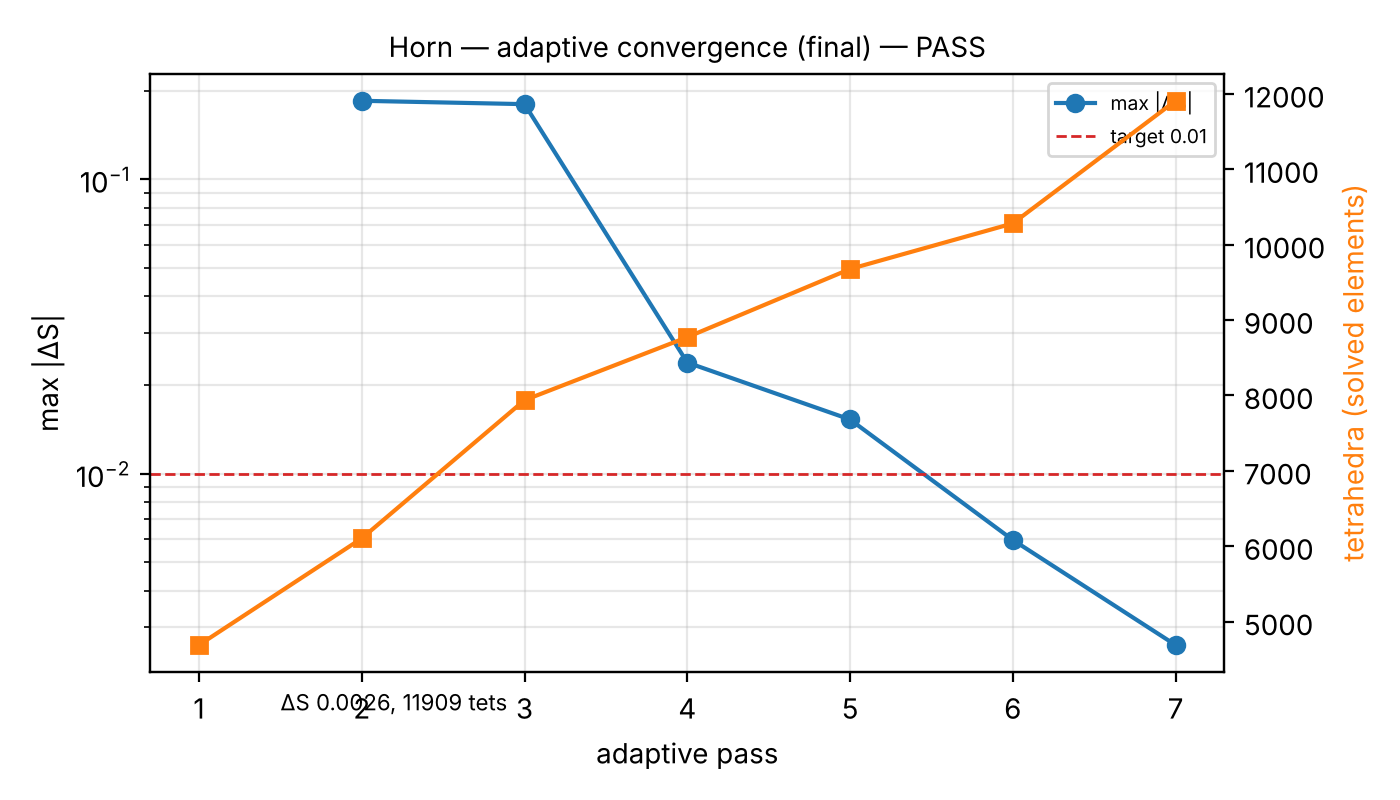
\includegraphics[width=0.85\linewidth,height=0.4\textheight,keepaspectratio]{figures/hfss/convergence}\caption{Mesh refinement}\end{figure}
\end{document}
